\documentclass{beamer}

\usepackage{natbib}

\usepackage[frenchb]{babel}

\usepackage[T1]{fontenc}

\usepackage[utf8]{inputenc}

\usepackage{amsmath}

\usepackage{tcolorbox}

\usepackage{lipsum}

\usepackage[labelformat=empty]{caption}

\usepackage{cclicenses}

\usetheme{Darmstadt}

\title{Hygiène cryptographique}

\author{\cc Ilan 'trog' Dubois}

\AtBeginSection[]
{
    \begin{frame}
        \frametitle{Sommaire}
            \tableofcontents[currentsection]
    \end{frame}
}

\begin{document}
    \begin{frame}
        \titlepage
    \end{frame}
    \section{Mb dszquphsbqijf}
    \subsection{Définitions}
        \begin{frame}{label=vocabulaire}
            \frametitle{Vocabulaire}
            \begin{center}
                \begin{itemize}
                    \item \textbf{Chiffrer}: Rendre incompréhensible un messgae pour qui n'aurait pas la clé.
                    \item \textbf{Déchiffrer}: Rendre à un message sa forme originale à l'aide de la clé.
                    \item \textbf{Décrypter}: Rendre à un message sa forme originale sans utiliser de clé (casser le code).
                    \begin{tcolorbox}[colback=green!5,colframe=green!40!black,title=Mais crypter alors ?]
                      En anglais chiffrer se dit \textit{encrypt}, d'où la confusion courante avec le terme \textit{crypter} qui en français signifie mettre dans une crypte.
                    \end{tcolorbox}
                \end{itemize}
            \end{center}
        \end{frame}
        \begin{frame}{label=utilisation}
            \frametitle{Les cas d'utilisation}
            \begin{center}
                \begin{itemize}
                    \item Rendre incompréhensible un document quelconque pour toute personne n'ayant pas la clé.
                    \item Assurer l'intégrité d'un document.
                    \item Assurer l'authenticité d'un document.
                \end{itemize}
            \end{center}
        \end{frame}
    \subsection{Deux principaux types de cryptographie}
        \begin{frame}{label=symmetric}
            \frametitle{La cryptographie symmétrique}
            \begin{center}
                \begin{itemize}
                    \item Chiffrement et déchiffrement se font avec une même clé.
                    \item César, Vigenaire, AES...
                    \item Est très rapide, utilisé pour chiffrer son disque, sa connexion...
                \end{itemize}
            \end{center}
        \end{frame}
        \begin{frame}{label=asymmetric}
            \frametitle{La cryptographie asymmétrique}
            \begin{center}
                \begin{itemize}
                    \item Utilise une paire de clé \textit{public}/\textit{privé}.
                    \item Le chiffrement se fait avec une clé publique. Le déchiffrement nécessite la clé privée.
                    \item DSA, RSA, Ed25519...
                    \item Plus lent mais aussi très pratique dans le cas où les parties ne partagent pas encore de \textit{secret}. Sert ainsi souvent à initier une connexion avec un chiffrement symmétrique.
                \end{itemize}
            \end{center}
        \end{frame}
        \begin{frame}
            \begin{center}
                \begin{figure}
                    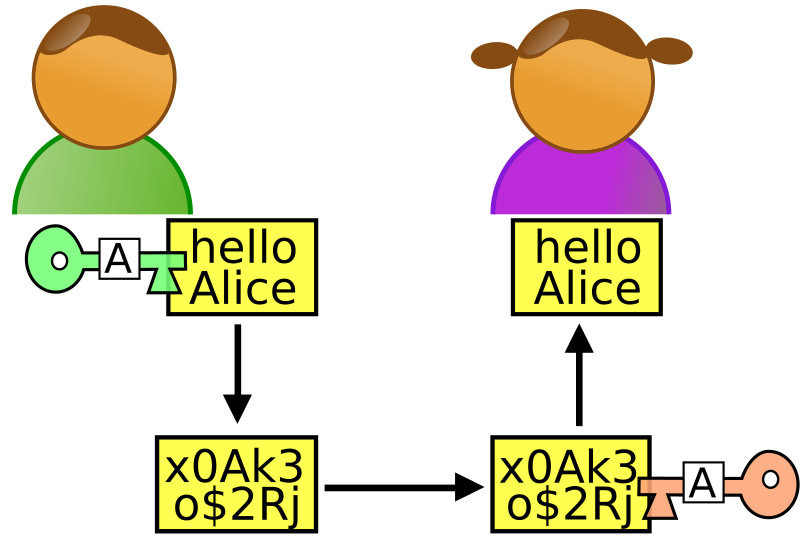
\includegraphics[scale=0.30]{img/asymmetric.png}
                    \caption{\cc --- odder}
                \end{figure}
            \end{center}
        \end{frame}
    \subsection{Un peu de pratique}
        \begin{frame}{label=cesar}
            \frametitle{Le chiffre de César}
            \begin{center}
                \begin{itemize}
                    \item Algorithme utilisé du temps de romains, son fonctionnement est très simple et réalisable à la main.
                    \pause
                    \item La clé est un nombre \textit{n} entre 1 et 25.
                    \pause
                    \item Pour chiffrer on remplace chaque lettre du message par la n-ième suivante dans l'alphabet.
                    \pause
                    \item Pour déchiffrer on remplace chaque lettre par la n-ième précédante.
                    \pause
                    \item César("Cryptographie", 3) \pause => Fubswrjudsklh
                \end{itemize}
            \end{center}
        \end{frame}
        \begin{frame}{label=attack}
            \frametitle{Décrypter César}
            \begin{center}
                \begin{itemize}
                    \item Approche \textbf{analytique}: la lettre la plus courante est "e". En observant quelle sont les lettres les plus courantes du message on déduit la clé.
                    \item Approche \textbf{bruteforce}: on essaie toutes les possibilités et on regarde ce qui semble être la réponse.
                    \item Ces deux approches sont dans le principe toujours celles utilisées aujourd'hui.
                \end{itemize}
                Let's practice !
            \end{center}
        \end{frame}
        \begin{frame}{label=fails}
            \frametitle{Epic fail}
            \begin{center}
                \begin{figure}
                    
\includegraphics[scale=0.15]{img/plain.jpg}
                    \caption{Image originale}
                \end{figure}
                \pause
                \begin{figure}
                    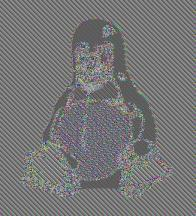
\includegraphics[scale=0.15]{img/aes_no_chain.jpg}
                    \caption{Chiffré sans chaînage}
                \end{figure}
                \pause
                \begin{figure}
                    
\includegraphics[scale=0.15]{img/aes_chain.jpg}
                    \caption{Chiffré avec chaînage}
                \end{figure}
                \cc --- Papa November \& Dr Juzam
            \end{center}
        \end{frame}
        \appendix
        \begin{frame}
            \bibliography{src/tracking}{}
            \bibliographystyle{plain}
        \end{frame}
\end{document}
